\setlength{\columnsep}{3pt}
\begin{flushleft}

\bigskip
\begin{itemize}
	\item \textbf{lsblk}: Lists information about all available block devices.
	
	\bigskip
	\begin{tcolorbox}[breakable,notitle,boxrule=-0pt,colback=pink,colframe=pink]
		\color{black}
		\fontdimen2\font=1em
		Syntax: lsblk
		\fontdimen2\font=4pt
	\end{tcolorbox}
	Eg:
	\begin{figure}[h!]
		\centering
		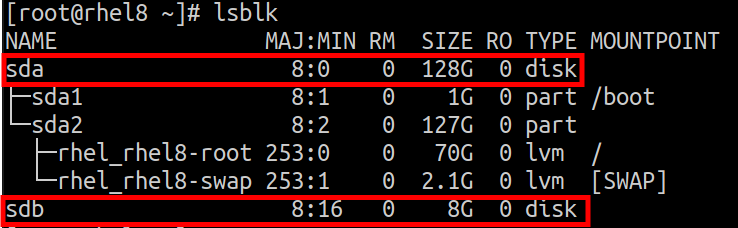
\includegraphics[scale=0.45]{content/chapter8/images/lsblk.png}
		\caption{lsblk command output}
		\label{fig:lsblk}
	\end{figure}
	
	\item \textbf{fdisk -l}: Display more detailed information about all disk drives.
	\bigskip
	\begin{tcolorbox}[breakable,notitle,boxrule=-0pt,colback=pink,colframe=pink]
		\color{black}
		\fontdimen2\font=1em
		Syntax: fdisk -l
		\fontdimen2\font=4pt
	\end{tcolorbox}
	Eg:
	\begin{figure}[h!]
		\centering
		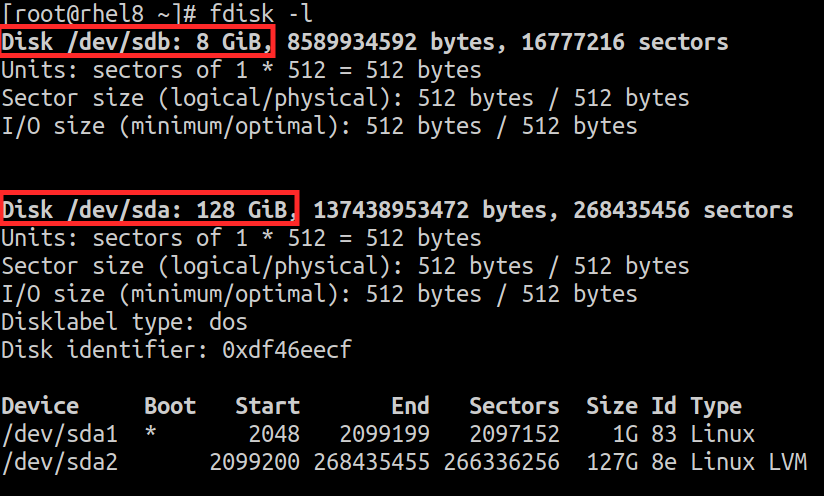
\includegraphics[scale=0.45]{content/chapter8/images/fdisk.png}
		\caption{"fdisk -l" command output}
		\label{fig:fdisk}
	\end{figure}
		
	
\end{itemize}
	
	
	
\end{flushleft}

\newpage

